%!TEX root = ../thesis.tex
%*******************************************************************************
%****************************** Metodologia *********************************
%*******************************************************************************

\chapter{Metodología}\label{chap:metod}

Este trabajo aplica una metodología de \textbf{integración continua y desarrollo colaborativo} de acuerdo con los objetivos del proyecto SIOSE-INNOVA y con un marco de trabajo actual aplicado tanto en el Laboratorio de Geomática de la Universidad de Alicante, como por otras empresas conocidas del sector (CARTO, Geographica, entre otros). En \citet{Zaragozi2017} se presentan distintos flujos de trabajo basados en esta metodología, los cuales están muy relacionados con lo que se expone en este capítulo y son de uso frecuente en el Laboratorio de Geomática. En las próximas páginas se presenta un flujo de trabajo para el desarrollo de una extensión de base de datos. No obstante, utilizando la misma metodología se pueden crear y mantener páginas web, realizar simulaciones con modelos geográficos o hasta se pueden crear documentos imprimibles (como este mismo trabajo).


\section{Integración continua y desarrollo colaborativo}

\begin{graybox}
\begin{itemize}
\item El trabajo colaborativo se ha coordinado utilizando \textit{Git} que es el sistema de \textbf{control de versiones} más popular de los últimos años (p.ej. utilizado en PostGIS, QGIS, CARTO y centenares de proyectos de ESRI, entre muchos otros).
\item La \textbf{contenerización o \textit{dockers}} es una novedosa tecnología para la virtualización de software/servicios, frente a la virtualización de sistemas operativos (p.ej. máquinas virtuales). La \textit{orquestación de dockers} permite organizar complejos sistemas de información con muchas facilidades.
\item PostgreSQL/PostGIS es la \textit{geodatabase libre} más potente del mercado, destacando por sus opciones de \textbf{extensibilidad} (p.ej. PostGIS en sí misma es una extensión de PostgreSQL).
\end{itemize}
\end{graybox}

El trabajo colaborativo ha sido fundamental en el desarollo de la extensión \pgland{} y por este motivo se dedica una parte importante de este trabajo a describir las herramientas colaborativas, bases de datos y técnicas que se ha aplicado para desarrollar y materializar los objetivos de este trabajo.

En esta sección se describen los procedimientos que se ha seguido periodicamente en este trabajo. La metodología de integración continua y el desarrollo colaborativo permiten colaborar con los miembros de un equipo de trabajo, lo cual asegura \textbf{un exhaustivo control de calidad y una mayor agilidad en la solución de problemas}.

En la subsección \ref{subsec:control} se describe el uso que se ha hecho de \textbf{\textit{Git}}, que es el sistema de control de versiones más popular de los últimos años. Siendo utilizado en un gran número de proyectos y empresas dedicadas a los SIG (p.ej. PostGIS\footnote{\href{https://github.com/postgis/postgis}{https://github.com/postgis/postgis}}, QGIS\footnote{\href{https://github.com/qgis/QGIS}{https://github.com/qgis/QGIS}}, CARTO\footnote{\href{https://github.com/CartoDB/cartodb}{https://github.com/CartoDB/cartodb}} y ESRI\footnote{\href{https://github.com/Esri}{https://github.com/Esri}}). A continuación, en la subsección \ref{subsec:conten-orquest} se presentan los servicios de contenerización o \textit{dockers} que se han utilizado para la virtualización del software/servicios necesarios para el desarrollo de la extensión, y la orquestación de éstos (despliegue sencillo de plataformas tecnológicas). La subsección \ref{subsec:exten} está dedicada a PostgreSQL, el Sistema Gestor de Bases de Datos (SGDB) \textit{libre} más potente del mercado y a su extensión espacial PostGIS. Finalmente, en la subsección \ref{subsec:aplic} se describen otras aplicaciones de escritorio que han sido utilizadas para analizar los resultados de esta metodología.


\subsection{Control de versiones}\label{subsec:control}

El control de versiones es la gestión de los cambios que se realizan sobre un archivo o conjunto de archivos en un repositorio y que se utiliza para controlar las versiones del código de fuente, de modo que se puedan recuperar versiones anteriores en un momento específico. Un repositorio es donde se almacenan todos los datos actualizados y los registros históricos de los cambios realizados, principalmente en un servidor.

El control de versiones se aplica hoy en día en muchas plataformas de uso cotidiano (p.ej. Dropbox, Gdocs, etc). Sin embargo, en proyectos profesionales se trabaja de forma colaborativa siguiendo una serie de pasos que aseguran que un usuario \textbf{no pueda sobrescribir el trabajo de otro compañero sin su consentimiento}. Esta dinámica consiste en que cada usuario modifica ficheros desde su máquina local, los guarda en Internet y luego propone los cambios al resto del equipo. El sistema de control combina las modificaciones \textbf{si todos los usuarios están de acuerdo}. En este trabajo se ha utilizado un software que permite trabajar de este modo:

\begin{itemize}
\item\textbf{Git}\footnote{La documentación referente a Git está disponible a través de la página oficial del proyecto (\url{https://git-scm.com/}).} es un sistema de control para el mantenimiento de versiones de código fuente de archivos. Git se ha convertido en la opción más popular de los últimos años y es utilizado por muchos proyectos como por ejemplo PostGIS, QGIS, CARTO y centenares de proyectos de ESRI, entre otros también muy conocidos. El control de versiones se realiza mediante una serie de verbos o instrucciones intuitivas como \textit{clone} (clonar un repositorio), \textit{pull} (traer cambios), \textit{push} (enviar cambios), \textit{add} (añadir nuevos ficheros) o \textit{commit} (registrar cambios en local), entre otras opciones menos habituales.
\item\textbf{GitHub}\footnote{La documentación de GitHub muestra distintos flujos de trabajo con Git así como documentación para distintas aplicaciones. Por ejemplo, es posible utilizar GitHub para crear una página web o una wiki (\url{https://github.com/}).} es una plataforma de desarrollo colaborativo que alberga proyectos y almacena el código fuente utilizando el sistema de control de versiones de \textit{Git}. Esto quiere decir que muchas de las tareas de Git pueden realizarse desde un navegador de Web de un modo sencillo. Además, GitHub es completamente gratuito a condición de que el código sea público, lo cual no es un problema en proyectos de software libre. En otras circunstancias, también existen otras plataformas similares como Bitbucket\footnote{\url{https://bitbucket.org}} o GitLab\footnote{\url{https://about.gitlab.com/}} con las que es posible que los repositorios privados sean gratuitos.
\end{itemize}

\begin{figure}
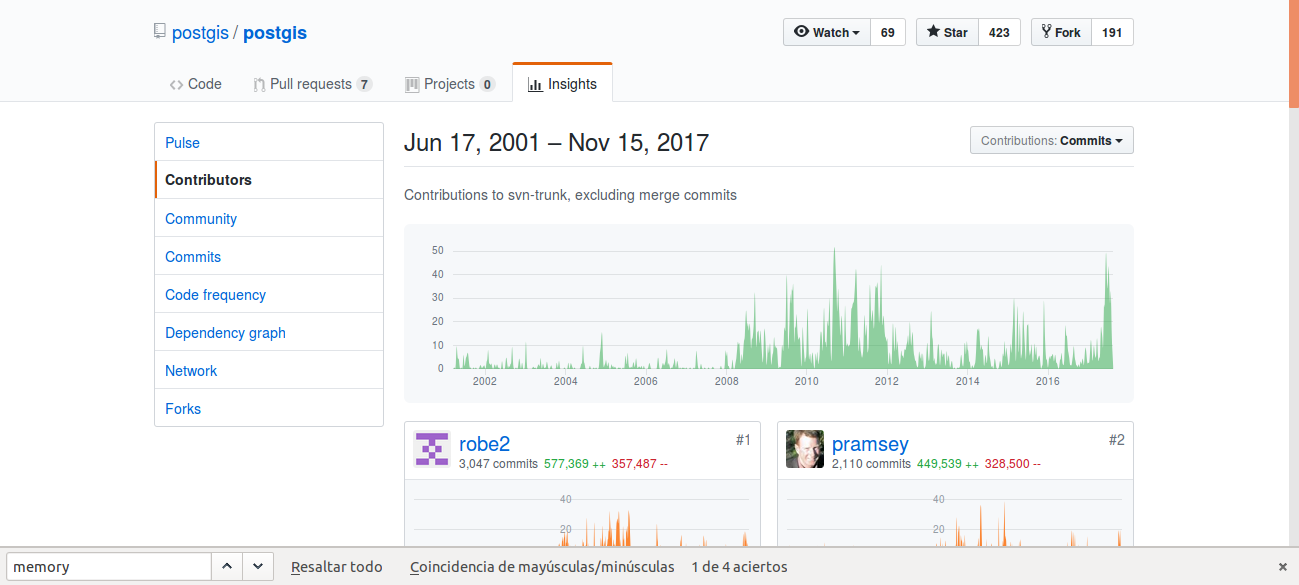
\includegraphics[width=\textwidth]{Metodologia/Figs/postgis-github}
\caption{Estadísticas de la comunidad de desarrolladores de PostGIS en la plataforma GitHub. Paul Ramsey es un desarrollador muy activo también en foros de usuarios. Fuente: \url{https://github.com/postgis/postgis}. \label{fig:postgis-github}}
\end{figure}

La extensión \pgland{}, principal objetivo de este trabajo, ha sido desarrollada y alojada en un repositorio personal y público en GitHub\footnote{\url{https://github.com/andrearosado/pg_landmetrics}}. Cuando se crean nuevas partes de la extensión, y funcionan correctamente, se proponen cambios al repositorio oficial del proyecto SIOSE-INNOVA\footnote{\url{https://github.com/siose-innova/pg_landmetrics}} y, si el resto de los colaboradores están de acuerdo, estos cambios pasan a formar parte de la versión oficial del proyecto.

El trabajo con Git es abierto y hay muchas maneras distintas de utilizar el software y colaborar con los otros usuarios. En el Laboratorio de Geomática de la Universidad de Alicante se trabaja como se detalla a continuación:

\begin{itemize}
\item El trabajo individual parte siempre de un \textbf{\textit{fork} del proyecto oficial}. Esto es un \textbf{\textit{repositorio remoto}} (en GitHub) idéntico, pero disociado del proyecto original en GitHub. Así es posible experimentar libremente para después compartir cambios o incluso derivar hacia un proyecto independiente. En cualquier caso la autoría del código seguirá siempre vinculada a sus creadores. En este punto, el usuario puede hacer un nuevo \textit{clone} local para trabajar desde un PC (\textbf{\textit{repositorio local}}).

\item \textbf{Actualización de ficheros de la extensión \pgland{} desde el repositorio local hacia el \textit{fork} en GitHub} (ver la figura \ref{fig:diary}). El procedimiento consiste en ejecutar el comando \textit{pull} desde la máquina local. Cuando el sistema de ficheros de la extensión no está actualizado, Git se encarga de obtener la última versión. Este paso es opcional, ya que si la versión local coincide con la remota, \textit{git pull} no tiene ningún efecto. Una vez el usuario recibe un mensaje de notificación de que su sistema de fichero estaba actualizado con la última versión, se puede proceder a editar los archivos de \pgland{}. Cuando la edición termina (p. ej. por que se ha añadido una nueva métrica), el usuario puede guardar los cambios utilizando los comandos \textit{git add} y \textit{git commit}. Al guardar estos cambios, Git proporciona un mensaje con un \textit{hash} (identificador único) por cada cambio que se haya realizado, o dicho de otro modo, se obtiene un identificador único para cada versión. Finalmente, desde la máquina local, el usuario sube esta última versión del la extensión a su repositorio del trabajo remoto (en GitHub), haciendo \textit{git pull}, con lo que la versión más reciente de su trabajo estaría en local y en su repositorio de GitHub (no el oficial).

\begin{figure}
\begin{center}
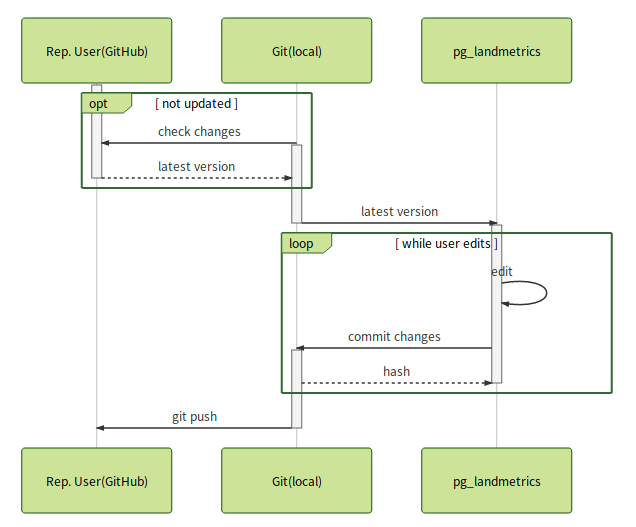
\includegraphics[width=0.9\textwidth]{Metodologia/Figs/diary.png}
\caption{Diagrama de secuencia en el que se describe el flujo de integración continua más habitual en este trabajo (varias veces al día). Cada vez que se realizaban cambios importantes en la extensión \pgland{}, se añadían al control de versiones local y al de \textit{La Nube de GitHub}. \label{fig:diary}}
\end{center}
\end{figure}

\item \textbf{Actualización de la extensión desde el repositorio del trabajo local hacia el repositorio oficial del proyecto SIOSE-INNOVA} (ver la figura \ref{fig:pullrequest}). Una de las primeras tareas de cualquier flujo de trabajo es realizar un \textit{fork}, es decir, una copia de todos los ficheros del repositorio oficial (\textit{upstream}) a un nuevo repositorio de este trabajo. La ventaja es que si en cualquier momento el repositorio \textit{copiado} sufriera algún contratiempo, se podría volver a conseguir una copia del repositorio oficial. Lo mismo ocurre con la versión local obtenida a partir del comando \textit{clone}. Éste último comando se ejecuta solamente cuando en la máquina local no existe una versión de \pgland{}. Esto implica que \textbf{siempre hay un mínimo de dos copias de respaldo con las que trabajar, además de todas las versiones anteriores}. A partir de este punto, se inicia el trabajo colaborativo entre usuarios y repositorios en GitHub. En este caso, se vuelve a repetir las mismas acciones de edición y actualización de archivos, como se ha visto en la Figura \ref{fig:diary}. Una vez subidos los cambios al \textit{fork} de GitHub, es posible enviar una petición al repositorio oficial (\textit{upstream}) para sincronizar ambos repositorios. Esta operación se denomina \textit{pull request} y permite compartir código entre repositorios alojados en la plataforma \textit{GitHub}. Si dicha petición (\textit{pull request}) es aceptada por el personal encargado del repositorio oficial (\textit{upstream}), se realiza una operación de unión (\textit{merge}) y se recibe una notificación de sincronización completada. En este punto, los repositorios en GitHub están casi sincronizados, salvo porque el repositorio oficial siempre cuenta con una nueva versión debida al \textit{pull request}. En el último paso, el usuario que ha efectuado solicitado el \textit{pull} descarga la última versión haciendo \textit{pull upstream} y subiendo los cambios a su versión en GitHub (\textit{fork}).

A pesar de lo complejo que parece este flujo de trabajo, se trata de \textbf{tareas sencillas y repetitivas en las que hay que comprobar que los cambios propuestos no son incompatibles con el trabajo anterior o de otros colaboradores}.

\begin{figure}
\begin{center}
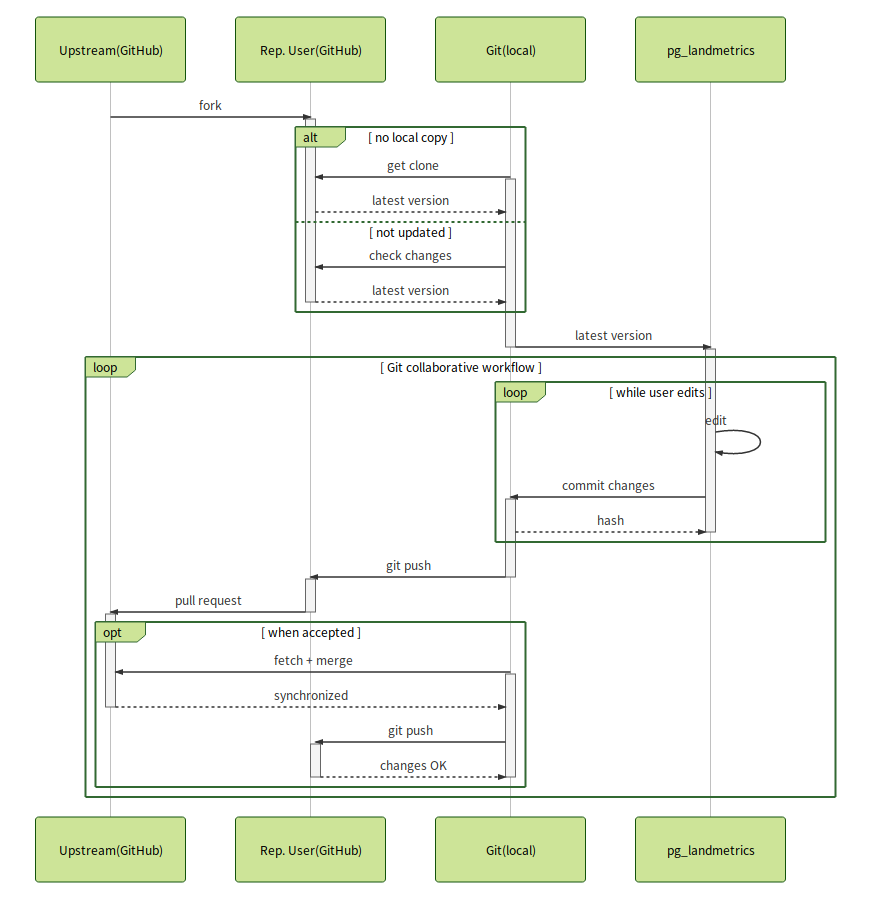
\includegraphics[width=0.9\textwidth]{Metodologia/Figs/pullrequest.png}
\caption{Diagrama de secuencia sobre el desarrollo colaborativo entre repositorios. Aproximadamente una vez al día, se proponen una serie de cambios al repositorio oficial (\textit{pull request}), si estos cambios son aceptados después es posible sincronizar los dos repositorios. \label{fig:pullrequest}}
\end{center}
\end{figure}

\end{itemize}






\subsection{Contenerización y orquestación de servicios}\label{subsec:conten-orquest}

La contenerización o \textit{docker} es una novedosa tecnología que aporta portabilidad y que \textbf{virtualiza aplicaciones y servicios frente a la virtualización de sistemas operativos completos (p. ej. máquinas virtuales}.

El trabajo con \textit{Dockers} es similar al trabajo con Git. Existen una serie de instrucciones o verbos que permiten construir (\textit{build}), desplegar (\textit{up}) o detener (\textit{down}) servicios que están empaquetados en contenedores (\textit{dockers}). Los contenedores son como ``cajas'' que contienen todo lo necesario para ejecutar una determinada aplicación o servicio. Los contenedores pueden trabajar aisladamente o conectados. La técnica que permite que los contenedores se conecten de una manera más sencilla se llama \textit{orquestación de contenedores} y es una técnica que permite organizar complejos sistemas de información con muchas facilidades. Existen distintas opciones de contenerización. Por ejemplo, la opción de Google se llama Kubernetes\footnote{\url{https://kubernetes.io/}}. Sin embargo en este trabajo se ha utilizado la plataforma más conocida que comprende varias herramientas de las que solamente presentamos las más importantes:

\begin{itemize}
\item\textbf{Docker}\footnote{\url{https://www.docker.com/}}: es un proyecto de código abierto que gestiona el despliegue de contenedores a través de \textit{La Nube}. Docker permite separar a las aplicaciones (\textit{software}) de la infraestructura (\textit{hardware}), a los desarrolladores del las tareas de mantenimiento, para crear un modelo colaborativo e innovador.
\item\textbf{Docker Hub}\footnote{\url{https://hub.docker.com/}}: es un servicio en la nube que permite vincular repositorios y crear y almacenar sus imágenes. Es una plataforma que centraliza y distribuye las imágenes en contenedores, además de facilitar la automatización en el proceso de desarrollo.
\item\textbf{Docker-compose}: utiliza un sencillo fichero de configuración que despliega todos los servicios necesarios de manera rápida y eficaz.
\end{itemize}

El uso de \textit{dockers} permite aplicar una metodología de integración continua a la hora de desarrollar e implementar una extensión como \pgland{} (ver la figura \ref{fig:ci}). El usuario no necesita trabajar directamente con \textit{dockers} sino que se puede automatizar en gran medida utilizando \textit{docker-compose}. Gracias a un \textit{software de orquestación} las pruebas sucesivas de la extensión se pueden realizar con un número mínimo de comandos: \textit{docker-compose build, up y down}

El comando \textit{docker-compose build} se utiliza únicamente si la extensión ha sido modificada (p. ej. al añadir una nueva métrica). En caso contrario no sería necesario volver a construir todos los contenedores, solamente se utilizaría el comando \textit{docker-compose up} para lanzar la última versión de la extensión. En el proyecto actual, la instrucción \textit{docker-compose up} se ocupa de lanzar dos contenedores: PostgreSQL/PostGIS y PgAdmin4. Una vez han sido lanzados dichos contenedores y se han recibido las notificaciones de que la conexión ha tenido éxito, \textbf{el usuario ya dispone de la última versión del SGBD con la última versión de \pgland{} instalada y acceso a los datos de ejemplo, todo ello con \textit{una única intrucción}}. Durante la \textit{orquestación} el SGBS y PgAdmin4 quedan conectados y configurados para empezar a trabajar en nuevas métricas del paisaje, las nuevas funciones creadas quedan guardadas en el sistema y es posible operar con Git como se ha explicado en la subsección \ref{subsec:control}. Una vez modificada la extensión y guardados los cambios en el control de versiones, todo el software utilizado se \textit{desinstala o se desmonta} con una única instrucción (\textit{docker-compose down}).

\begin{figure}
\begin{center}
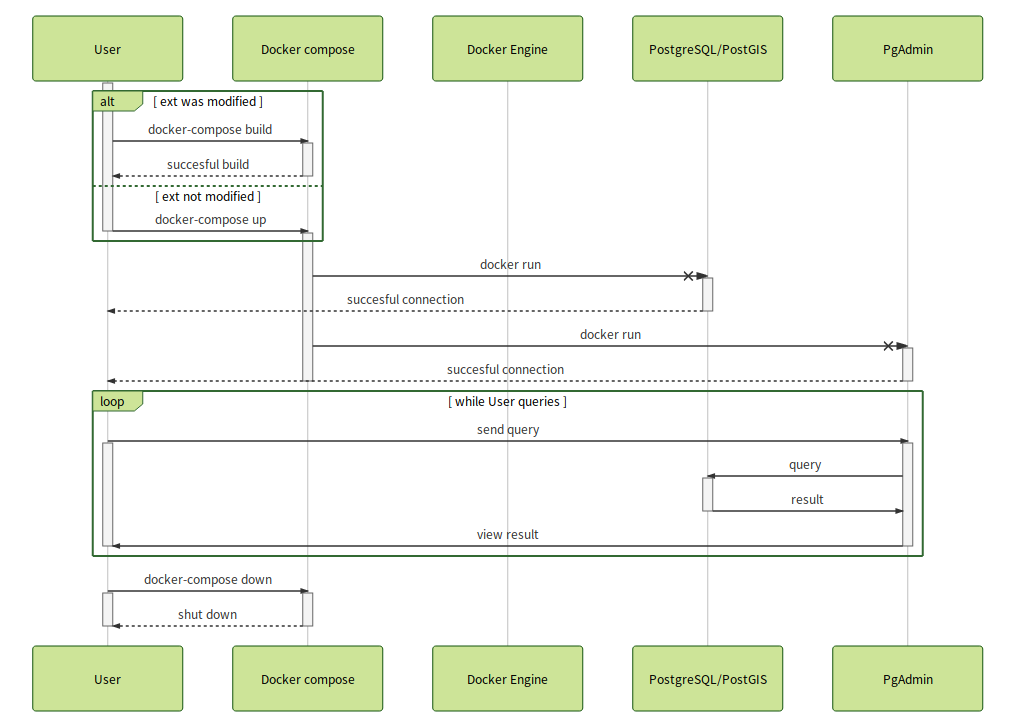
\includegraphics[width=\textwidth]{Metodologia/Figs/ci.png}
\caption{Diagrama de secuencia. Integración continua en la implementación y desarrollo de funciones SQL con \textit{dockers}. Cada vez que una nueva función es añadida a la base de datos, se elimina cualquier rastro de la versión anterior y se vuelve a lanzar un nuevo contenedor para evaluar si los cambios son válidos. \label{fig:ci}}
\end{center}
\end{figure}


\subsection{Extensibilidad en PostgreSQL}\label{subsec:exten}

PostgreSQL, y su extensión espacial PostGIS, fueron utilizados en las asignaturas del Máster a un nivel de usuario, lo cual ha resultado muy útil en la creación de funciones y métricas. En este trabajo se han utilizado las últimas versiones de estos programas en el momento de realizar los experimentos (PostgreSQL 9.6 y PostGIS 2.3). En el desarrollo de las prácticas se han estudiado otras ventajas de estas tecnologías. Sin embargo, en este trabajo hay que destacar una de las características más notables de este SGBD: la extensibilidad.

La \textit{extensibilidad} es la adaptabilidad de un \textit{software} frente a la introducción de nuevos cambios y funcionalidades. En este sentido PostgreSQL es un SGBD altamente extensible, ya que \textbf{toda su funcionalidad se añade como si de un catálogo se tratase}. El sistema de tipos, funciones, índices, operadores y funciones agregadas, son solo algunas de las características que pueden ser extendidas en PostgreSQL. Este diseño extensible ha servido para crear el propio PostGIS, que es una \textit{extensión}. Una extensión de Postgres sería un conjunto de nuevas funcionalidades que son añadidas de manera conjunta. Además, de las características ya mencionadas, los propios lenguajes procedurales serían extensiones en cierto modo. Lo más interesante es que estas extensiones se pueden programar en cualquiera de los lenguajes disponibles en PostgreSQL, incluido SQL.

Físicamente, una extensión de PostgreSQL consiste en varios ficheros que automatizan la instalación en una base de datos de nuevos tipos de datos, funciones, operadores (espaciales o no), funciones agregadas, entre otros objetos\footnote{La creación de extensiones en PostgreSQL es relativamente sencilla pero tiene muchas opciones (ver \href{https://www.postgresql.org/docs/10/static/extend-extensions.html}{https://www.postgresql.org/docs/10/static/extend-extensions.html})}. \textbf{La mayor parte de aportaciones de este trabajo al proyecto SIOSE-INNOVA encajan en este punto, creando funciones y funciones agregadas, (en su mayor parte en lenguaje SQL), para ser incorporadas en la extensión \pgland{}.}

La plataforma de contenerización descrita en la subsección \ref{subsec:conten-orquest} realiza muchas tareas de instalación y configuración. Entre estas tareas, la más significativa consiste en la instalación automática de la última versión de la extensión a partir de un fichero \textit{makefile} en el que se organiza todo el código de la extensión\footnote{GNU Make es un software muy conocido para automatizar la compilación de nuevos programas de un modo determinado. PostgreSQL hace un uso particular de esta tecnología para facilitar la instalación de extensiones pero para saber más es posible consultar la documentación oficial en \href{https://www.gnu.org/software/make/manual/make.html}{https://www.gnu.org/software/make/manual/make.html}}. Junto con el desarrollo de código SQL, la actualización de este fichero es esencial para que la extensión se instale correctamente.


\subsection{Otras aplicaciones}\label{subsec:aplic}

La mayor parte de este trabajo se ha realizado utilizando Git, Dockers y PostgreSQL, que funcionan como servicios y no necesitan de un interfaz gráfico para operar. Dado el carácter abierto y multiplataforma de estas aplicaciones, el Sistema Operativo tampoco es una limitación (Linux GNU, Windows o Mac). Sin embargo, hay tareas en las cuales contar con un interfaz gráfico bien organizado puede resultar de gran ayuda.

La preparación de datos de ejemplo y la visualización de las consultas realizadas con PostgreSQL se han realizado con las siguientes aplicaciones:

\begin{itemize}
\item\textbf{PgAdmin4}\footnote{\url{https://www.pgadmin.org/}}: es una plataforma que administra, gestiona y desarrolla código abierto en bases de datos PostgreSQL. En la Figura \ref{fig:carga} se muestra una captura de pantalla de PgAdmin4 mientras se realiza una carga masiva de datos procedentes del SIOSE. Cabe decir que en el Máster se trabajo con la versión anterior de este programa, la funcionalidad es muy similar aunque cambie el aspecto, pero el despliegue con Dockers hace que la instalación de este programa en cualquier ordenador sea más sencilla y que pueda funcionar también desde un servidor de Internet.
\item\textbf{QGIS 2.18}\footnote{\url{https://www.qgis.org/es/site/}}: es una aplicación de escritorio SIG, de código abierto, que analiza, maneja y opera con datos como \textit{raster/vector} y bases de datos. Además, facilita la conexión entre bases de datos espaciales como PostGIS. Este programa ya se conocía ampliamente, aunque en este trabajo se ha trabajado fundamentalmente con el gestor de bases de datos y la visualización de geometrías provenientes de PostgreSQL/PostGIS.
\end{itemize}

\begin{figure}
\begin{center}
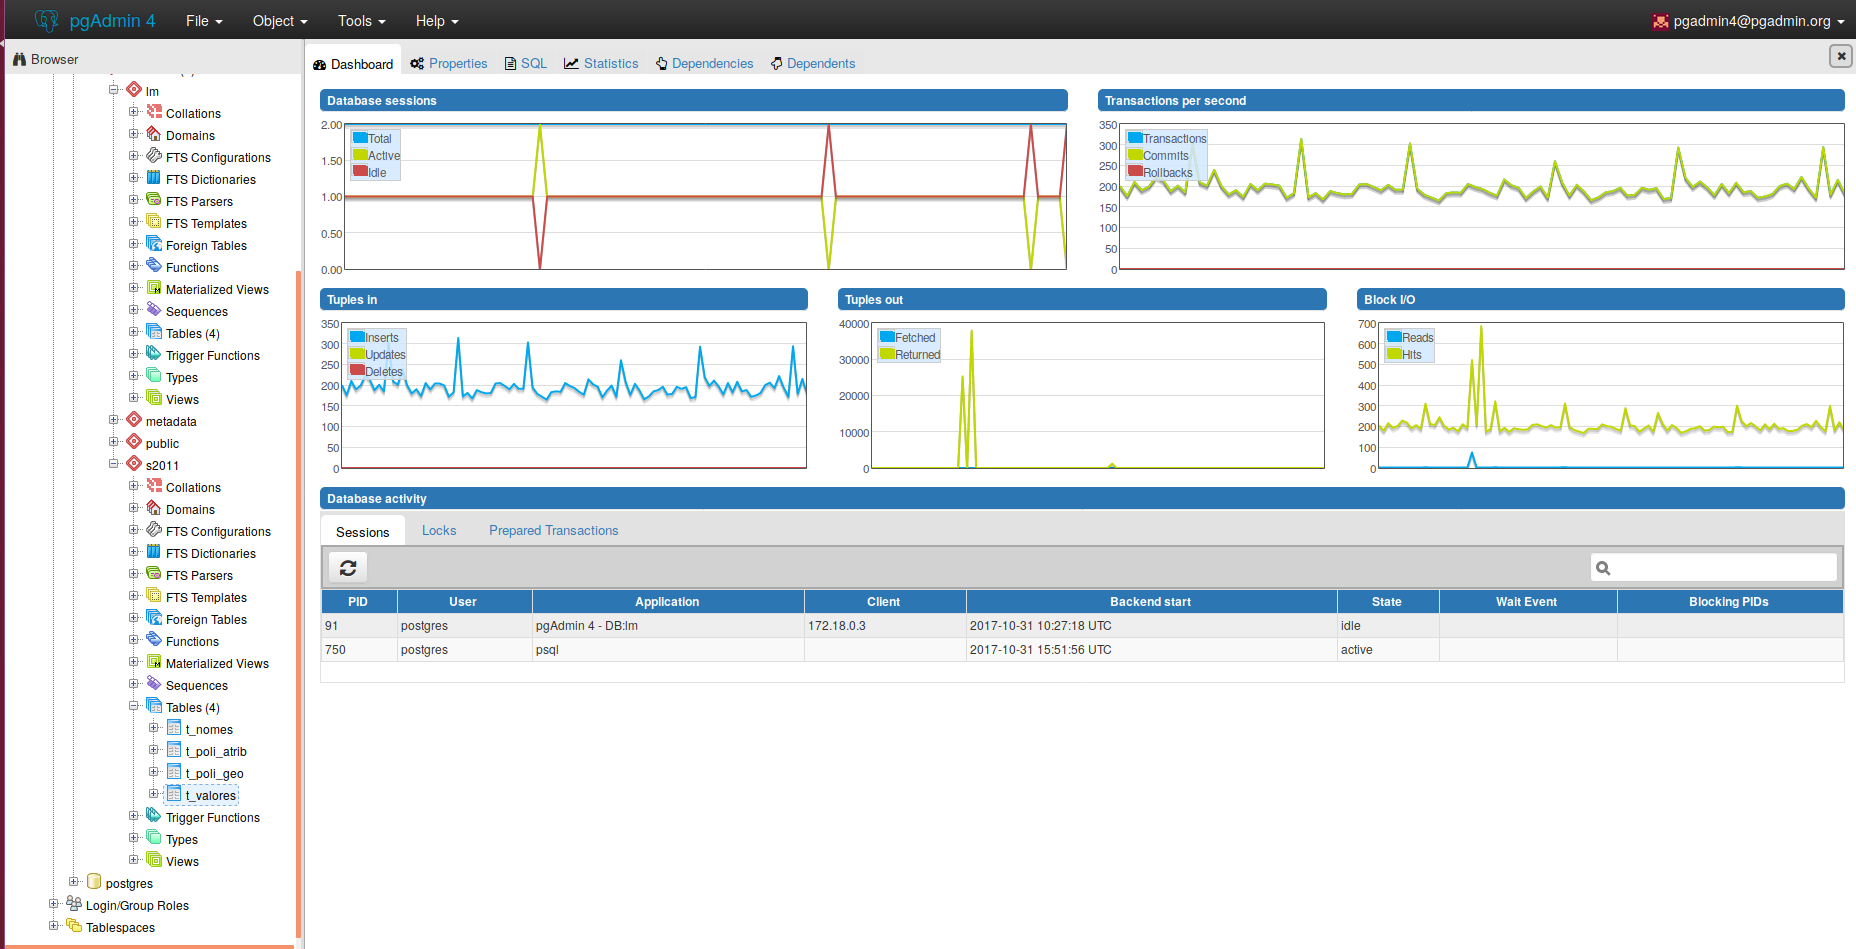
\includegraphics[width=\textwidth]{Metodologia/Figs/carga-siose-2011.png}
\caption{Vista de la interfaz web de PgAdmin4. Fuente: \url{http://localhost:5050/browser/}. \label{fig:carga}}
\end{center}
\end{figure}


\section{Conjuntos de datos\label{sec:datos}}

\begin{graybox}

En este trabajo se han utilizado los siguientes conjuntos de datos:

\begin{itemize}
\item \textbf{Un capa con un paisaje de ejemplo} para comprobar que la extensión \pgland{} da resultados correctos para las métricas.
\item \textbf{La base de datos SIOSE-2011} para realizar una prueba de capacidad de consulta sobre un gran volumen de datos.
\item Varios \textbf{grids a distintas escalas} (1:25.000, 1:50.000, 1:100.000 y 1:500.000) para simular una serie de consultas por parte de un usuario (ver ejemplo de la Figura \ref{fig:visorweb}).

\end{itemize}
\end{graybox}

En esta sección se describen los dos conjuntos de datos utilizados para poner a prueba la extensión \pgland{}: un paisaje de ejemplo y el SIOSE de 2011.

El \textbf{paisaje de ejemplo} se ha utilizado para comprobar si las métricas de paisaje funcionan correctamente, comparando los resultados ofrecidos desde PgAdmin4, como también desde QGIS (DB-Manager). La escala de digitalización para esta capa es 1:50.000 y se ha creado en dos sistemas geodésicos de referencia: European Terrestrial Reference System 1989 (ETRS89) y World Geodetic System 84 (WGS84), ya que las métricas no se calculan igual si se trabaja con geometrías proyectadas (\textit{geometry}) o si se utiliza un sistema de coordenadas esféricas (\textit{geography}). 

En este pequeño conjunto de datos hay un total de 51 polígonos que se han digitalizado utilizando las herramientas de edición avanzada y geoproceso de QGIS. Se han definido 8 categorías de cobertura de suelo donde a cada polígono le corresponde un tipo de categoría representada por un color (ver figura \ref{fig:zona_andrea}). Se han definido los colores a partir de los 147 que recoge la Scalable Vector Graphics (SVG) Specification\footnote{\url{http://www.december.com/html/spec/colorsvg.html}} además de tener en cuenta la clasificación de color que especifica el \textit{Corine Land Cover (CLC)}.

\begin{figure}
\begin{center}
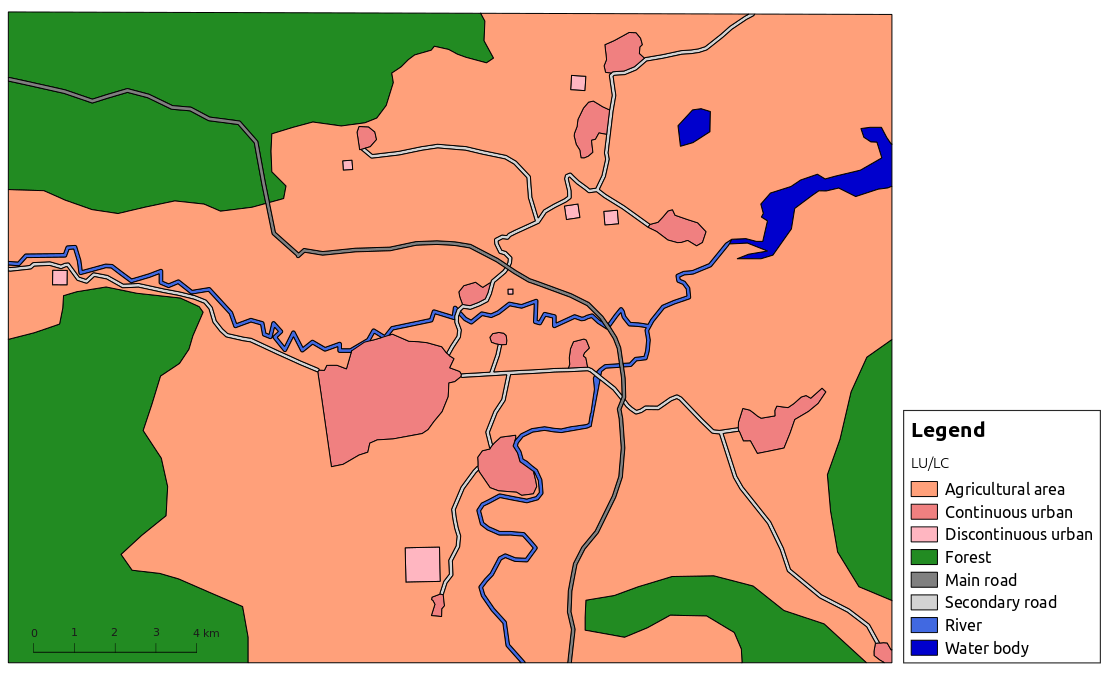
\includegraphics[width=\textwidth]{Metodologia/Figs/zona_andrea.png}
\caption{Coberturas del suelo del paisaje de ejemplo. Estas geometrías se distribuyen junto con la extensión \pgland{} para que los usuarios realicen pruebas antes de importar sus propios datos. \label{fig:zona_andrea}}
\end{center}
\end{figure}

El segundo conjunto de datos que se ha utilizado es la base de datos \textbf{SIOSE 2011} facilitada por el Servicio de Ocupación del Suelo del Instituto Geográfico Nacional (IGN), gracias a su participación en el proyecto SIOSE-INNOVA. Cabe decir que esta base de datos contiene más información y es más compleja que la versión descargable desde el Centro de Descargas del Centro Nacional de Información Geográfica.

Esta base de datos tan voluminosa se compone de 4 tablas. En la tabla de datos \texttt{t\_nomes} se encuentran todas las nomenclaturas de cada polígono, en \texttt{t\_poli\_atrib} todos los atributos de los polígonos como por ejemplo el código multietiqueta de clasificación del SIOSE o de clasificación de las distintas nomenclaturas (iberpix, perfil ambiental, toponimia, \textit{Corine Land Cover}, etc.), en cuanto a la tabla \texttt{t\_poli\_geo} ofrece la geometría de cada uno de los 2.562.800 de polígonos existentes y, finalmente, en la tabla \texttt{t\_valores} aparecen los valores de coberturas y usos del suelo codificados y asociados a los polígonos, así como también cálculos de valores en Hectáreas.

Como se menciona en la sección \ref{sec:siose}, los polígonos del SIOSE pueden describirse por una \textit{cobertura simple} o una \textit{cobertura compuesta}. Dentro de esta última se encuentran las coberturas no predefindidas, es decir, que un mismo polígono puede contener varías coberturas de suelo. A raíz de esta característica, se ha realizado una reclasificación de los polígonos a partir de la cobertura prevalente que presenta la jerarquización de la clasificación de los usos y coberturas del suelo del SIOSE. Con ello se ha obtenido una nueva tabla con 85 coberturas prevalentes asignadas a cada uno de los polígonos que se encuentran en la tabla \texttt{t\_poli\_geo}. Para que las consultas sean más rápidas entre las distintas tablas se han generado índices para indexar los datos de cada una de las tablas. Esta reclasificación es necesaria ya que trabajar con clasificaciones \textit{multietiqueta} de usos y coberturas del suelo es un problema más amplio que no se pretende abordar en este trabajo.

Una vez se han reclasificado todos los polígonos del SIOSE-2011, se han obtenido \textbf{\textit{grids}} (cuadrículas cartográficas) para el cálculo de métricas del paisaje a distintas escalas de referencia, a través del Centro de Descargas del Instituto Geográfico Nacional (CNIG)\footnote{\url{http://centrodedescargas.cnig.es/CentroDescargas/index.jsp}}.

A partir del grid 1:500.000 se han escogido dos celdas de las zonas de estudio en las cuales se han calculado algunas métricas de paisaje. Estas dos zonas contienen la mayor parte de las provincias de Alicante y Zaragoza, así como los alrededores de cada una\footnote{Se han escogido estas dos zonas es por hacer referencia al lugar donde se han realizado las prácticas de empresa y dónde se ha cursado el \textit{máster}.}. A continuación se han seleccionado y extraído todas aquellas celdas que comprenden las dos celdas de las áreas de estudio con escala de referencia 1:25.000, 1:50.000 y 1:100.000. A partir de todas estas celdas ha simulado una serie de consultas como las que podrían darse en un visor web. La Figura \ref{fig:visorweb} ayuda a visualizar en que consiste la simulación o experimento que se analiza en el capítulo \ref{chap:result}.


% Please add the following required packages to your document preamble:
% \usepackage{booktabs}
% \usepackage{multirow}
\begin{table}[]
\centering
\caption{Características de los conjuntos de datos utilizados. \label{tab:datos}}
\begin{tabular}{@{}llll@{}}
\toprule
\textbf{Tipo}               & \textbf{Tablas} & \textbf{Filas} & \textbf{Tamaño total} \\ \midrule
\multirow{4}{*}{SIOSE-2011} & t\_nomes        & 36.790.972     & 6116 MB               \\
                            & t\_poli\_atrib  & 2.562.800      & 451 MB                \\
                            & t\_poli\_geo    & 2.562.800      & 3981 MB               \\
                            & t\_valores      & 10.932.639     & 1041 MB               \\ \midrule
\multirow{4}{*}{Grids}      & grid\_25k       & 756            & 232,3 kB              \\
                            & grid\_50k       & 192            & 57,8 kB               \\
                            & grid\_100k      & 48             & 13,8 kB               \\
                            & grid\_500k      & 2              & 677bytes              \\ \midrule
\multirow{2}{*}{Sample}     & sample\_25830   & 51             & 122,6 kB              \\
                            & sample\_4326    & 51             & 122,5 kB              \\ \bottomrule
\end{tabular}
\end{table}


\section{Selección de métricas}\label{sec:metricas}

\begin{graybox}
\begin{itemize}
\item El número potencial de métricas del paisaje es \textbf{muy amplio} y depende de muchos factores (p.ej. objetivos del estudio, modelos de datos como \textit{raster/vector} o en red, niveles de agregación y/o escala, etc).
\item Resulta esencial determinar unas \textbf{métricas representativas} para esta primera propuesta.
\end{itemize}
\end{graybox}

Como se indica en la sección \ref{sec:metrica}, existen cientos de métricas de paisaje que no siempre tienen significado para todas las aplicaciones de estudio, ya que su interés depende de muchos factores (p. ej. los objetivos del estudio, el modelo de datos, la escala, nivel de agregación etc). Por este mismo motivo y según los objetivos de este trabajo, se han seleccionado unas métricas del paisaje representativas y que aparecen frecuentemente en la bibliografía consultada.

En la tabla \ref{tab:listmetricas} se listan las métricas acompañadas por su abreviatura. Se ha escogido un número de métricas repartidas por igual en tres niveles de agregación: a nivel de polígono (\textit{patch}), nivel de categoría (\textit{class}) y nivel de paisaje (\textit{landscape}). Además, se han escogido métricas que calculan operaciones simples, como por ejemplo el área o el perímetro, y por otro lado, métricas cuyos cálculos son más complejos, como por ejemplo la distancia al vecino más próximo o la densidad. El objetivo ha sido encontrar la mayor variedad posible de contratiempos en el desarrollo de nuevas métricas.

% Please add the following required packages to your document preamble:
% \usepackage{multirow}
\begin{table}[]
\centering
\caption{Métricas de paisaje disponibles en la extensión.}
\label{tab:listmetricas}
\begin{tabular}{lll}
\hline
\textbf{Nivel}             & \textbf{Métrica}                     & \textbf{Abreviatura} \\ \hline
\multirow{8}{*}{Patch}     & Patch Area                           & AREA                 \\
                           & Patch Perimeter                      & PERIM                \\
                           & Perimeter-Area-Ratio                 & PARA                 \\
                           & Shape Index                          & SHAPE                \\
                           & Core Area                            & CORE                 \\
                           & Number of Core Areas                 & NCORE                \\
                           & Core Area Index                      & CAI                  \\
                           & Euclidean Nearest Neighbour Distance & ENN                  \\ \hline
\multirow{8}{*}{Class}     & Total (Class) Area                   & CA                   \\
                           & Percentage of Landscape              & PLAND                \\
                           & Total Edge                           & TE                   \\
                           & Edge Density                         & ED                   \\
                           & Total Core Area                      & TCA                  \\
                           & Core Area Percentage of Landscape    & CPLAND               \\
                           & Number of Patches                    & NP                   \\
                           & Patch Density                        & PD                   \\ \hline
\multirow{9}{*}{Landscape} & Total Area                           & TA                   \\
                           & Total Edge                           & TE                   \\
                           & Edge Density                         & ED                   \\
                           & Number of Patches                    & NP                   \\
                           & Patch Density                        & PD                   \\
                           & Patch Richness                       & PR                   \\
                           & Patch Richness Density               & PRD                  \\
                           & Shannon's Diversity Index            & SHDI                 \\
                           & Simpson's Diversity Index            & SHIDI                \\ \hline
\end{tabular}
\end{table}


\section{Desarrollo de funciones en PostgreSQL}

\begin{graybox}
\begin{itemize}
\item Los desarrollos en PostgreSQL se pueden realizar en lenguajes de programación como ANSI C, SQL y/o distintos lenguajes procedurales (p.ej. PL/pgSQL, PL/R, PL/Python, entre muchos otros), \textbf{dependiendo de las necesidades}.
\item El lenguage SQL es el más sencillo para programar en PostgreSQL y está mejor integrado.
\end{itemize}
\end{graybox}

La implementación y desarrollo en PostgreSQL se puede realizar desde distintos lenguajes de programación como por ejemplo ANSI C que es un estándar del lenguaje de programación C. Es el más popular en el desarrollo de softwares y aplicaciones, y además su código es portable entre distintas plataformas. Otro de los lenguajes de programación más conocido y utilizado hasta la fecha es \textbf{SQL (\textit{Structured Query Language})}. Es un lenguaje de consulta estructurada en gestión de bases de datos relacionales que maneja algébra y cálculo relacional. Este tipo de lenguaje es declarativo ya que ofrece la posibilidad de realizar consultas para obtener un resultado, además de estar orientados a resolver problemas. Finalmente, PostgreSQL da la posibilidad de utilizar distintos lenguajes procedurales para realizar tareas que en SQL resulten demasiado complicadas. El lenguaje procedural más habitual es PL/pgSQL, pero también hay otros como PL/R, PL/Python, o PL/Bash que permiten programar en la base de datos utilizando una gran variedad de recursos de análisis.


Dado que se ha trabajado sobre una base de datos relacional y orientada a objetos como es la del SIOSE y se ha utilizado tanto PgAdmin4 como la extensión de PostgreSQL/PostGIS, se ha empleado como lenguaje de programación SQL en la mayoría de los casos para simplificar o compactar lo máximo posible todas las funciones de la extensión y que éstas no dependan de otras. SQL es un lenguaje estandarizado y resultaría viable migrar estas consultas a otros SGBD como Oracle Spatial o SQLite. Además, el motor de consultas de PostgreSQL solamente puede ser aprovechado al máximo al ejecutar SQL, siendo las funciones de otros lenguajes procedurales como ``cajas negras'' que impiden optimizar más las consultas. Sin embargo, es cierto que en algunos casos se ha tenido que emplear PL/pgSQL cuando no era posible elaborar las funciones en SQL.

Una vez decidido qué lenguaje de programación utilizar para implementar y desarrollar las funciones, se han construido consultas SQL a partir de las métricas seleccionadas (ver Tabla \ref{tab:listmetricas}). Las fórmulas de estas métricas han sido extraídas de la documentación del software FRAGSTATS, que es referencia para otros programas mencionados en la introducción. Los resultados de cada consulta SQL se validaron manualmente sobre el conjunto de datos de ejemplo, utilizando QGIS para calcular las métricas por pasos.

Cuando estas últimas comprobaciones han resultado satisfactorias, se ha procedido a desarrollar la función de PostgreSQL por cada una de las métricas. Cabe mencionar que todas las funciones se han desarrollado por duplicado, para calcular las métricas proyectadas (\textit{geometry}) o en coordenadas esféricas (\textit{geography}). Así pues, la extensión permite trabajar con conjuntos de datos con prácticamente cualquier sistema geodésico de referencia.

Dentro de las opciones que permite PostgreSQL hay métricas que se han podido implementar como \textbf{funciones simples}, pero en otros casos ha sido necesario crear \textbf{funciones agregadas} más complejas.

\subsubsection{Funciones simples}

Las funciones simples corresponden a las métricas de paisaje a nivel de polígono. Como ejemplo de ello, la métrica de paisaje \textit{Patch Area (AREA)} devuelve la suma del área del polígono dividido por 10.000 para obtener un valor en unidades de hectárea. Como se puede observar en el ejemplo de código (\ref{area1}), a partir de la fórmula matemática que calcula esta métrica, se ha construido su consulta SQL, la cual resulta sencilla de leer.

\lstset{caption=Consultas SQL para la métrica AREA.,label=area1}
\begin{SQL}
SELECT St_Area(geom)/10000 FROM sample_patches_25830;
SELECT St_Area(geom)/10000 FROM sample_patches_4326;
\end{SQL}


Una vez escrita una consulta SQL (ejemplo \ref{area1}), se puede desarrollar una función de un modo bastante estructurado. Como se observa en el ejemplo de código \ref{area2}, la función se define a partir del nombre de la propia función, el tipo de valor que devuelve, la consulta SQL que se ha construido anteriormente y finalmente, un comentario en el que explica lo que la función tiene que devolver como resultado. Como se ha mencionado anteriormente, la función se ha elaborado tanto para \textit{geometry} como para \textit{geography}, ya que PostGIS lo permite.

\lstset{caption=Función simple para calcular la métrica AREA por polígonos.,label=area2}
\begin{SQL}
CREATE OR REPLACE FUNCTION p_area(geom geometry)
RETURNS metric AS 
$$

SELECT (1, St_Area(geom)/10000)::metric;

$$
LANGUAGE SQL
IMMUTABLE
RETURNS NULL ON NULL INPUT;

COMMENT ON FUNCTION p_area(geom geometry) IS 'Divide el área en metros cuadrados de un polígono por 10.000 para devolver un valor en Hectáreas.';
\end{SQL}


Una vez se ha creado la función, se valida el resultado devuelto a través de un ejemplo de uso. Por ejemplo, en el ejemplo de código \ref{area3}) se calcula la métrica AREA a para todo el conjunto de datos de ejemplo.

\lstset{caption=Ejemplo de uso para calcular la métrica AREA.,label=area3}
\begin{SQL}
SELECT (p_area(geom)).value As p_area FROM sample_patches_25830;
SELECT (p_area(geom)).value As p_area FROM sample_patches_4326;
\end{SQL}



\subsubsection{Funciones de agregación}

No todas las métricas se pueden calcular como funciones simples de PostgreSQL. Las funciones simples aplican un cálculo individualmente a filas o polígonos de la base de datos. Cuando una métrica implica un sumatorio y/o operaciones entre varias filas o polígonos (diversidad, vecindad, etc), entonces es necesario utilizar funciones de agregación. Normalmente, todas las métricas a nivel de categoría o a nivel de paisaje serán funciones de agregación. Por ejemplo, las funciones SUM() o COUNT() de PostgreSQL, son algunas de las más utilizadas, pero \textbf{como se ha dicho en la subsección \ref{subsec:exten} es posible extender PostgreSQL/PostGIS con funciones de agregación propias.}

A modo de ejemplo, la métrica \textit{Total Core Area (TCA)} devuelve la suma de los núcleos de las áreas (m$ ^{2} $) de cada polígono, dividido por 10.000 (para obtener Hectáreas). Al igual que en el ejemplo de código \ref{area1}, se ha preparado una nueva consulta basada en la función matemática utilizada en FRAGSTATS. En el ejemplo de código (\ref{tca1}) se aprecian que en este caso es necesario específicar una \textit{profundidad de borde} (un buffer negativo) para calcular la métrica.

\lstset{caption=Consulta SQL para la métrica TCA.,label= IDW1}
\begin{SQL}
SELECT SUM(St_Area(St_Buffer(geom, -50)))/10000 FROM sample_patches_25830;
SELECT SUM(St_Area(St_Buffer(geom, -50)))/10000 FROM sample_patches_4326;
\end{SQL}


A partir de ésta consulta (ver ejemplo \ref{tca1}), se ha desarrollado la función de agregado. La diferencia que tiene esta función respecto a la de \textit{Patch Area} es que se necesita crear un agregado dentro de la función ya que el resultado que se quería obtener era agrupado según el tipo de categoría. Como se observa en el ejemplo de código \ref{tca2}, la función se estructura por el nombre de la propia función, el tipo de valor que devuelve que en este caso será etiquetado el resultado según el tipo cobertura de suelo al que corresponde, la consulta SQL que se ha construido anteriormente desglosada de distinta forma que la anterior ya que se quería obtener el sumatorio del resultado de los polígonos agrupados por categoría, un agregado que forma la estructura del resultado con el valor y la etiqueta de cobertura, y finalmente, un comentario en el que explique qué tiene que devolver como resultado. Como se ha mencionado, la función se ha elaborado tanto para \textit{geometry} como para \textit{geography}.

\lstset{caption=Función de agregado para calcular TCA por categorías.,label=lst:tca2}
\begin{SQL}
CREATE OR REPLACE FUNCTION c_totalcorearea_state(
	current_state metric_labeled,
	geom geometry,
	category text)
    RETURNS metric_labeled
    LANGUAGE 'sql'

AS 
$BODY$

WITH inputs AS (
    	SELECT current_state AS cstate
), melt AS (
    	SELECT unnest((cstate).pairs) AS m2 FROM inputs
    	UNION 
	SELECT (category, (p_corearea(geom)).value)::metric_labeled_pair AS m2
), summarize AS (
	SELECT (m2).label, SUM((m2).value) AS value FROM melt GROUP BY (m2).label
)
SELECT (13, ARRAY(SELECT (label, value)::metric_labeled_pair FROM summarize))::metric_labeled;

$BODY$;

CREATE AGGREGATE c_totalcorearea(geometry, text)(
    SFUNC=c_totalcorearea_state,
    STYPE=metric_labeled,
    INITCOND='(13,{})'
);

COMMENT ON AGGREGATE c_totalcorearea(geom geometry, category text) IS 'Suma las áreas de los núcleos de cada polígono de la misma categoría dividido por 10.000 para devolver un valor en Hectáreas.';
\end{SQL}





Una vez se ha desarrollado la función de agregado, se ha ejecutado un ejemplo de uso (ver ejemplo de código \ref{tca3}) para obtener el cálculo de la métrica TCA a partir de un conjunto de datos (ver en la figura \ref{fig:fig_ejemplo}).

\begin{figure}
\begin{center}
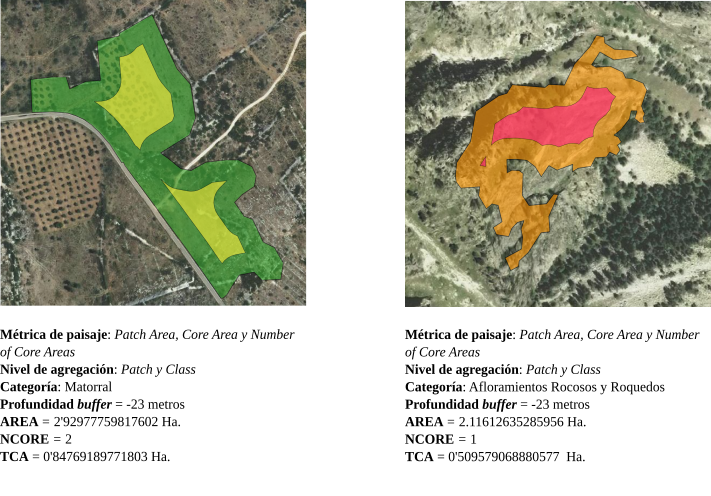
\includegraphics[width=\textwidth]{Metodologia/Figs/figuraejemplo.png}
\caption{Ejemplo de cálculo de AREA, NCORE y TCA a partir de la geometría del SIOSE 2011. \label{fig:fig_ejemplo}}
\end{center}
\end{figure}

\lstset{caption=Crear una función para calcular el IDW (I),label= IDW1}
\begin{SQL}
SELECT c_totalarea(geom,category) FROM sample_patches_25830;
SELECT c_totalarea(geom,category) FROM sample_patches_4326;
\end{SQL}


En cuanto a las métricas a nivel de paisaje también se han desarrollado de tipo agregado para obtener \textbf{un solo resultado para el conjunto de todo el paisaje}. A partir de este punto, se han elaborado todas las funciones de las métricas que se han seleccionado en la sección \ref{sec:metricas}.

\section{Experimento sobre la capacidad de cálculo de \pgland{}\label{sec:exp}}

Una vez todas las funciones han sido desarrolladas, implementadas y testeadas sobre el conjunto de datos de ejemplo, resulta sencillo realizar pruebas de rendimiento de la extensión \pgland{} sobre el conjunto de datos del SIOSE-2011.

\textbf{Este experimento busca simular la consulta que un usuario podría realizar en un visor web del SIOSE que calculase métricas del paisaje de un modo ágil e interactivo (ver figura \ref{fig:visorweb}).} Cada vez que el usuario hace zoom o se desplaza por el visor Web SIG, se envían consultas sobre las métricas del paisaje para la superficie del mapa visible en ese momento (normalmente será una superficie rectangular). 

El movimiento del usuario se simula a partir de una secuencia de consultas utilizando como referencia los grids descritos en la sección \ref{sec:datos}. En este sentido se ha colaborado en la elaboración de una última función (ajena a la extensión) para automatizar la realización de numerosas consultas sobre el SIOSE-2011 (ver ejemplo de código \ref{list:runtests}). Los resultados de este experimento se explican en el capítulo \ref{chap:result}.

\lstset{caption=Extracción de los resultados de las métricas en diferentes escalas de referencia a partir de grids.} \label{list:runtests}
\begin{SQL}
CREATE OR REPLACE FUNCTION test.runtests() 
  RETURNS TABLE ( 
    grid_tablename regclass,
    zone_id int,
    cell_id int,
    total_landscape_area numeric,
    avg_patch_area numeric,
    total_class_area numeric) 
LANGUAGE 'plpgsql'
AS $$ 
DECLARE
  script text;

BEGIN 
  SELECT DISTINCT string_agg('SELECT * from test.runtests(' || quote_literal(table_schema || '.' || table_name) || ')', ' UNION ALL ') into script
  FROM information_schema.tables where table_schema = 'test' and table_name like 'grid_%';

  RETURN QUERY EXECUTE script;

END
$$;
\end{SQL}
\label{list:runtests}

Esta función construye una tabla virtual con los resultados organizados por columnas según la zona de estudio a la que corresponden (Zaragoza o Alicante), el número de celda sobre el que está intersectado, y los valores de cada métrica en su columna correcta. A continuación se ha ejecutado un \textit{script}, proporcionado por el personal del Laboratorio de Geomática, el cual extrae todos los valores calculados, para todas las escalas de referencia y en una sola tabla en formato CSV.

Resulta importante destacar que este experimento sobre la extensión \pgland{} se ha desarrollado en un ordenador de sobremesa, con Sistema Operativo Ubuntu 17.10 (64 bits), 7,7 GB de memoria, un procesador Intel Core i7-7700 CPU @ 6.60 GHz x 8 y con un disco duro de 1,2 TB. No se ha realizado ninguna configuración fuera de las opciones estándar de PostgreSQL.


\section{Documentación de la extensión}

\begin{graybox}
\begin{itemize}
\item Una parte fundamental de esta metodología es la \textbf{documentación} del desarrollo y uso de la extensión. 
\item Una buena documentación con ejemplos facilitará el cálculo de métricas del paisaje en grandes repositorios, \textbf{sobretodo para aquellos usuarios con menos experiencia} en PostgreSQL/PostGIS.
\end{itemize}
\end{graybox}

La documentación del desarrollo y uso de la extensión es una de las partes más importante de la metodología de este trabajo. Una buena documentación facilitará el despliegue y aprovechamiento de la extensión a otros usuarios, sobretodo a aquellos menos expertos en la materia. La documentación ha consistido en introducir de manera sistemática comentarios en el código de la extensión (documentación para desarrolladores) y en crear documentos de apoyo (documentación para usuarios).

La documentación de proyectos también se presta a aplicar una metodología de integración continua y a trabajar en plataformas colaborativas. Ha sido necesario aprender a manejar distintos \textbf{lenguajes de marcado} (tipo HTML) para los distintos tipos de documentos:

\begin{itemize}
\item\textbf{Markdown para documentación Web}\footnote{\url{https://github.com/adam-p/markdown-here/wiki/Markdown-Cheatsheet}}. Markdown es un lenguaje ligero que permite una escritura sencilla y de fácil lectura usando texto plano. Se ha utilizado para documentar el uso de la extensión en GitHub.
\item\textbf{TeX para documentación en PDF}\footnote{\url{https://www.latex-project.org/}}. TeX es el lenguaje que se utiliza en el sistema de textos LaTeX y que crea documentos con una alta calidad tipográfica. Desde hace tiempo este lenguaje se emplea por un gran número de usuarios para escribir artículos o libros científicos. Para trabajar con este lenguaje, se ha utilizado la aplicación Texmaker. Este trabajo ha sido creado en formato PDF mediante el uso de estos programas.
\item\textbf{Scalable Vector Graphics (SVG) para la generación de gráficos vectoriales a partir de las geometrías de PostGIS}\footnote{\url{https://www.w3schools.com/graphics/svg_intro.asp}}. SVG es un lenguaje capaz de crear gráficos basados en vectores escalables de alta calidad de resolución. A partir de este lenguaje se ha desarrollado una función capaz de representar gráficos vectoriales a partir de las geometrías de cualquier geodatabase (ver en el anexo \ref{anex:svg}).
\item\textbf{Mermaid para la creación de diagramas}.\footnote{\url{https://mermaidjs.github.io/}} Mermaid es un lenguaje que genera gráficos a partir de texto mediante JavaScript. Se han generado desde diagramas de flujo, diagramas de secuencia y de Gantt. Algunos de los cuales se encuentran el la página Web del GitHub.
\end{itemize}
